%%%%%%%%%%%%%%%%%%%%%%%%%%%%%%%%%%%%%%%%%%%%%%%%%%%%%%%%%%%%%%%%%%%%%%%%%%%%%%%%
%%%%%%%%%%%%%%%%%%   Vorlage für eine Abschlussarbeit   %%%%%%%%%%%%%%%%%%%%%%%%
%%%%%%%%%%%%%%%%%%%%%%%%%%%%%%%%%%%%%%%%%%%%%%%%%%%%%%%%%%%%%%%%%%%%%%%%%%%%%%%%

% Erstellt von Maximilian Nöthe, <maximilian.noethe@tu-dortmund.de>
% ausgelegt für lualatex und Biblatex mit biber

% Kompilieren mit 
% latexmk --lualatex --output-directory=build thesis.tex
% oder einfach mit:
% make

\documentclass[
  tucolor,       % remove for less green,
  BCOR=12mm,     % 12mm binding corrections, adjust to fit your binding
  parskip=half,  % new paragraphs start with half line vertical space
  open=any,      % chapters start on both odd and even pages
  cleardoublepage=plain,  % no header/footer on blank pages
]{tudothesis}


% Warning, if another latex run is needed
\usepackage[aux]{rerunfilecheck}

% just list chapters and sections in the toc, not subsections or smaller
\setcounter{tocdepth}{1}

%------------------------------------------------------------------------------
%------------------------------ Fonts, Unicode, Language ----------------------
%------------------------------------------------------------------------------
\usepackage{fontspec}
\defaultfontfeatures{Ligatures=TeX}  % -- becomes en-dash etc.

% german language
\usepackage{polyglossia}
\setdefaultlanguage{german}

% for english abstract and english titles in the toc
\setotherlanguages{english}

% intelligent quotation marks, language and nesting sensitive
\usepackage[autostyle]{csquotes}

% microtypographical features, makes the text look nicer on the small scale
\usepackage{microtype}

%------------------------------------------------------------------------------
%------------------------ Math Packages and settings --------------------------
%------------------------------------------------------------------------------

\usepackage{amsmath}
\usepackage{amssymb}
\usepackage{mathtools}

% Enable Unicode-Math and follow the ISO-Standards for typesetting math
\usepackage[
  math-style=ISO,
  bold-style=ISO,
  sans-style=italic,
  nabla=upright,
  partial=upright,
]{unicode-math}
\setmathfont{Latin Modern Math}

% nice, small fracs for the text with \sfrac{}{}
\usepackage{xfrac}  


%------------------------------------------------------------------------------
%---------------------------- Numbers and Units -------------------------------
%------------------------------------------------------------------------------

\usepackage[
  locale=DE,
  separate-uncertainty=true,
  per-mode=symbol-or-fraction,
]{siunitx}
\sisetup{math-micro=\text{µ},text-micro=µ}

%------------------------------------------------------------------------------
%-------------------------------- tables  -------------------------------------
%------------------------------------------------------------------------------

\usepackage{booktabs}       % \toprule, \midrule, \bottomrule, etc

%------------------------------------------------------------------------------
%-------------------------------- graphics -------------------------------------
%------------------------------------------------------------------------------

\usepackage{graphicx}
% currently broken
% \usepackage{grffile}

% allow figures to be placed in the running text by default:
\usepackage{scrhack}
\usepackage{float}
\floatplacement{figure}{htbp}
\floatplacement{table}{htbp}

% keep figures and tables in the section
\usepackage[section, below]{placeins}


%------------------------------------------------------------------------------
%---------------------- customize list environments ---------------------------
%------------------------------------------------------------------------------

\usepackage{enumitem}

%------------------------------------------------------------------------------
%------------------------------ Bibliographie ---------------------------------
%------------------------------------------------------------------------------

\usepackage[
  backend=biber,   % use modern biber backend
  autolang=hyphen, % load hyphenation rules for if language of bibentry is not
                   % german, has to be loaded with \setotherlanguages
                   % in the references.bib use langid={en} for english sources
]{biblatex}
\addbibresource{references.bib}  % the bib file to use
\DefineBibliographyStrings{german}{andothers = {{et\,al\adddot}}}  % replace u.a. with et al.


% Last packages, do not change order or insert new packages after these ones
\usepackage[pdfusetitle, unicode, linkbordercolor=tugreen]{hyperref}
\usepackage{bookmark}
\usepackage[shortcuts]{extdash}

%------------------------------------------------------------------------------
%-------------------------    Angaben zur Arbeit   ----------------------------
%------------------------------------------------------------------------------

\author{Maximilian Nöthe}
\title{\LaTeX-Dokumentenklasse und Vorlage für Abschlussarbeiten an der TU Dortmund}
\date{2014}
\birthplace{Castrop-Rauxel}
\chair{Lehrstuhl für Experimentelle Physik V}
\division{Fakultät Physik}
\thesisclass{Bachelor of Science}
\submissiondate{31. September 2015}
\firstcorrector{Prof.~Dr.~Erstgutachter}
\secondcorrector{Prof.~Dr.~Zweitgutachter}

% tu logo on top of the titlepage
\titlehead{
\includegraphics[height=1.5cm]{logos/tu-logo.pdf}}

\begin{document}
\frontmatter
\thispagestyle{empty}
\setcounter{page}{2}
\section*{Hinweise}
Empfohlen wird die Verwendung dieser Vorlage mit der jeweils aktuellsten TeXLive Version (Linux, Windows) bzw. MacTeX Version (MacOS).
Aktuell ist dies TeXLive 2016. Download hier:
\begin{center}
  \ttfamily\url{https://www.tug.org/texlive/}
\end{center}
Bei Verwendung von TexLive Versionen 2014 und älter sollte
die Zeile
\begin{center}
\verb+\RequirePackage{fixltx2e}+ 
\end{center}
als erste Zeile der Präambel noch vor der Dokumentenklasse eingefügt werden.
Dies lädt diverse Bugfixes für LaTeX, die ab TexLive 2015 Standard sind.

Die Vorlage \texttt{thesis.tex} ist für die Kompilierung mit \texttt{lualatex} ausgelegt, mit wenigen Anpassungen kann sie aber auch mit \texttt{pdflatex} oder \texttt{xelatex} verwendet werden. 
Die Dokumentenklasse \texttt{tudothesis.cls} kann mit allen drei Programmen verwednet werden.

Achten Sie auch auf die Kodierung der Quelldateien.
Bei Verwendung von Xe\LaTeX\ oder Lua\LaTeX\ (empfohlen) müssen die
Quelldateien UTF-8 kodiert sein.
Bei Verwendung von pdf\LaTeX\ nutzen Sie die Pakete \texttt{inputenc} und \texttt{fontenc} mit der korrekten Wahl der Kodierungen.

Eine aktuelle Version dieser Vorlage steht unter 
\begin{center}
  \ttfamily\url{https://github.com/maxnoe/tudothesis}
\end{center}
zur Verfügung.

Alle verwendeten Pakete werden im \LaTeX{} Kurs von Pep et al.\ erklärt:
\begin{center}
  \ttfamily\url{http://toolbox.pep-dortmund.org/notes}
\end{center}

Für Rückmeldungen und bei Problemen mit der Klasse oder Vorlage, bitte ein \emph{Issue} auf GitHub aufmachen oder eine Email an
\href{mailto:maximilian.noethe@tu-dortmund.de}{maximilian.noethe@tu-dortmund.de} schreiben.

Wenn Sie die Dokumentenklasse mit der Option \texttt{tucolor} laden, werden verschiedene Elemente in TU-Grün gesetzt.

\maketitle

% Gutachterseite
\makecorrectorpage

% hier beginnt der Vorspann, nummeriert in römischen Zahlen
\thispagestyle{plain}
\nocite{PhysRevLett.121.221802}

\section*{Abstract}
\begin{english}
Differential measurement of the $tq\gamma$ process in the Standard Model would enable investigations of the electromagnetic coupling of the top quark. 
Regarding this measurement of $tq\gamma$ with the full Run-2 dataset at the ATLAS experiment, a neural network is trained on data from Monte Carlo simulations to discriminate background processes from the $tq\gamma$ signal process. 
Certain features of events are provided as input to the neural network. 
In this thesis, the influence of these input features on the neural network's ability to separate signals from the background is investigated. This provides insights into which event features are essential characteristics to understand the electromagnetic coupling of the top quark.
\end{english}

\tableofcontents

\mainmatter
% Hier beginnt der Inhalt mit Seite 1 in arabischen Ziffern
\chapter{Introduction}
Hier folgt eine kurze Einleitung in die Thematik der Bachelorarbeit.
Die Einleitung muss kurz sein, damit die vorgegebene Gesamtlänge der 
Arbeit von 25 Seiten nicht überschritten wird. 
Die Beschränkung der Seitenzahl sollte man ernst nehmen,
da Überschreitung zu Abzügen in der Note führen kann. 
Um der Längenbeschränkung zu genügen, darf auch nicht an der Schriftgröße,
dem Zeilenabstand oder dem Satzspiegel (bedruckte Fläche der Seite) manipuliert werden.

\chapter{Single top quark production with a photon in the Standard Model}
\section{A brief overview of the standard model}
\section{The \texorpdfstring{$tq\gamma$}{TEXT} process in the standard model}
\chapter{Measurement of \texorpdfstring{$tq\gamma$}{TEXT}}
\section{The ATLAS Experiment}
\section{Object Reconstruction at the ATLAS experiment}
\section{Background contributions from similar processes}
\chapter{Monte Carlo samples and event selection}
\section{Generation of Monte Carlo samples}
\section{Event selection}
\chapter{The Neural Network used for signal-background classification}
\section{The NN model}
\section{}
\chapter{Analysis of the effects of different event properties on the neural network output}
\section{Correlations of input data with the NN output}
\section{Changes in event distribution of the NN output for different phpt and fjphmae bins}
\chapter{Conclusions}

\chapter{Single top quark production with a photon in the Standard Model}
\section{A brief overview of the standard model}
\section{The \texorpdfstring{$tq\gamma$}{tqGamma} process in the standard model}


\chapter{Measurement of \texorpdfstring{$tq\gamma$}{tqGamma}}



\section{The ATLAS Experiment}

The European Organization for Nuclear Research, known as CERN, located in Geneva, has various experiments studying elementary particles through the collision of heavy ions and protons. 
The Large Hadron Collider (LHC), the particle accelerator of CERN, has a circumference of $27 \si{\kilo\metre}$ and can collide particles with an energy of up to $13.6 \si{\tera\electronvolt}$. 


The LHC consists of four extensive experiments: the ALICE, the LHCb, the CMS and the ATLAS experiments. The research in this paper is done with the help of the largest of these experiments, the ATLAS experiment. Figure 1 visualizes the structure of the ATLAS detector.  The detector is built symmetrically around the particle beam divided into three subdetectors.

The inner detector tracks charged particles just after the collision. It consists of three different systems of sensors in a magnetic field parallel to the beam. These sensors are the pixel detector, the semiconductor tracker that works with silicon strips and a transition radiation tracker to track particles with gas-filled tubes. 

In the EM calorimeter, metal layers (tungsten, copper or lead) absorb incoming particles and convert them into lower-energy particles called a shower. The calorimeters detect "showers" produced by electrons, photons and hadrons. 
Hadrons do not deposit all of their energy into the EM calorimeter; they get absorbed by steel layers in the hadronic calorimeter. 
Plastic scintillating tiles then produce photons that get converted into an electric current. 

The muon spectrometer measure trajectories of muons with the help of a magnetic field. The spectrometer detects muons in the range of $\bigl|\eta\bigr| = 2.7$. 
Monitored drift tubes measure for pseudorapidities up to $\eta = 2.0$ and cathode strip chambers fill higher pseudorapidities.  
\begin{figure}
    \centering
    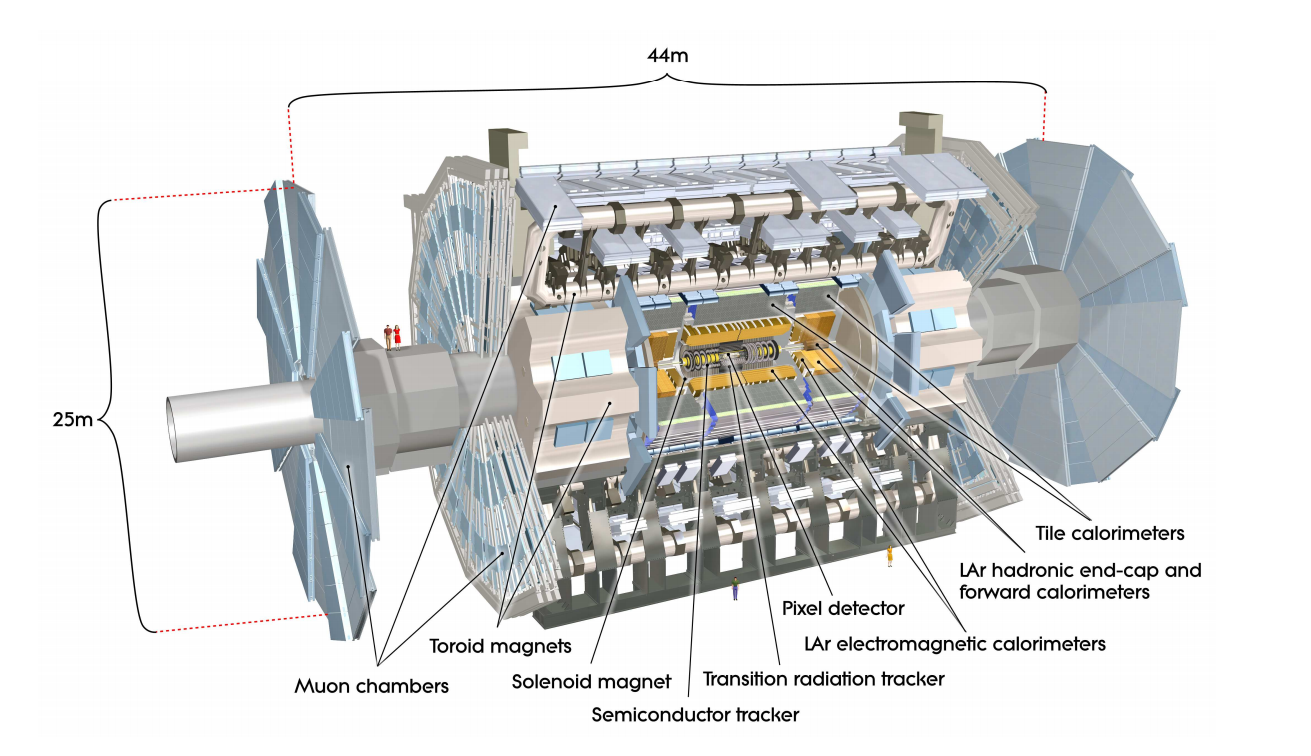
\includegraphics[width=0.9\textwidth]{Plots/atlasSCHEMA.PNG}
    \label{fig:atlasschema}
    \caption{Schematic visualisation of the ATLAS Detector \cite{Collaboration_2008}.}
\end{figure}



\section{Object Reconstruction at the ATLAS experiment}

\subsection{Reconstruction of photons}


\subsection{Reconstruction of leptons}
\subsection{Jets}

Jets are clusters of mostly mesons that result from the separation of two quarks. They are reconstructed with the help of the anti-$k_t$ algorithm with a radius parameter of R = 0.4 \cite{anti_k_t}. 
This algorithm reconstructs jets by first identifying the particle source via the jet energy scale. It is then required that the jet has a transverse momentum of $p_T > 25 \si{\giga\electronvolt}$ and $\bigl|\eta\bigr| < 4.5$. 

Detector noise can lead to the misidentification of a jet. The nature of these misidentified jets has been studied thoroughly \cite{70} and a so-called "jet cleaning procedure" is used to tag them. 
Any event containing at least one "bad" jet is removed. 



\section{Background contributions from similar processes}


The criteria for event selection \ref{sec:eventselect} allow various different processes besides $tq\gamma$. These events contribute to the background noise. Any process that has similar decay products as tqGamma are background. 
The process $t\bar{t}\gamma$ holds the most similar decay product as it's products can be identical to the products of $tq\gamma$. Following processes is the production of a $W$-boson with jets, a $Z$-boson with jets and $t\bar{t}$. 
Table \ref{tab:background} lists these and the rest of the processes contributing to the background.
\begin{table}
    \centering
    \begin{tabular}{c c c}
        \toprule
        {} & Process \\
        \midrule
        1 & $tq\gamma$\\[.1cm]
        2 & $t\bar{t}\gamma$\\[.1cm]
        3 & $W\gamma + jets$\\[.1cm]
        4 & $Z\gamma + jets$\\[.1cm]
        5 & $t\bar{t}$\\[.1cm]
        6 & $s\-chan$\\[.1cm]
        7 & $t W$\\[.1cm]
        8 & $t\-chan$\\[.1cm]
        9 & $VV$\\[.1cm]
        10& $W+jets$\\[.1cm]
        11& $Z+jets$\\[.1cm]
        \bottomrule
    \end{tabular}
    \caption{List of SM processes that contribute to background noise in the measurement of $tq\gamma$.}
    \label{tab:background}
\end{table}



\chapter{Monte Carlo samples and event selection}
\section{Generation of Monte Carlo samples}
\section{Event selection}
\chapter{The Neural Network used for signal-background classification}
\section{Short introduction to neural networks}
\section{The neural network architecture}
\section{Input features for the neural network}
\section{Performance and distribution of the NN output}
\chapter{Analysis of the effects of different event features on the neural network output}
\section{Correlations of input features with the NN output}
\section{Changes in the NN output distribution for different photon \texorpdfstring{$p_T$}{TEXT} and fjet+photon energy bins}
\section{?}
\chapter{Conclusions}
\chapter{Abbildungen und Tabellen}

\section{Abbildungen}

Achten Sie bei ihren Plots auf ausreichend große Achsenbschriftungen, ausreichende Schriftdicken und gut unterscheidbare Farben.
Im Idealfall haben Sie im Plot und der Arbeit die gleiche Schriftgröße und Schriftart.
Dies lässt sich durch Erstellen des Plots in der korrekten Größe und Einbinden mit dem optionalen Argument \texttt{scale=1} erreichen. Ein Beispiel sehen Sie in Abbildung \ref{fig:bsp}.

Nutzen Sie wenn möglich Vektorgrafiken (pdf) und nur in Ausnahmen Rastergrafiken wie .png oder .jpg.
Setzen Sie Punkte hinter Abbildungsunterschriften.

\begin{figure}
    \centering
    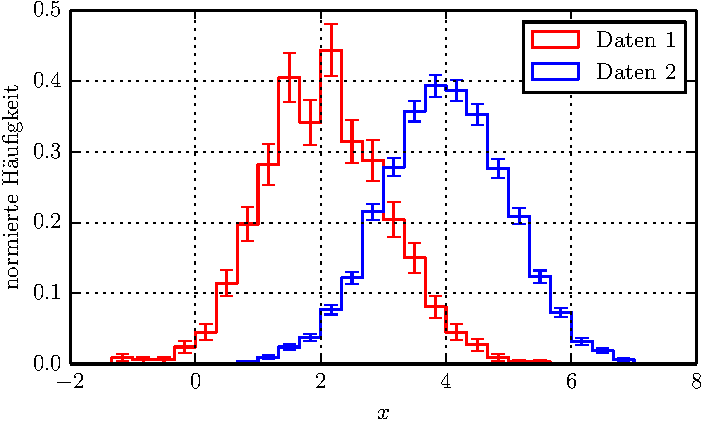
\includegraphics[scale=1]{./Plots/Histogramm.pdf}
    \caption{Ein Histogramm mit Fehlerbalken für zwei Datensätze, Schriftgröße und -art entsprechen der des Dokuments.}
    \label{fig:bsp}
\end{figure}

\section{Tabellen}

Tabellen sollten so einfach wie möglich aufgebaut sein, verzichten Sie auf zu viele Linien. In fast allen Fällen reichen drei horizontale Linien aus, jeweils über und unter der Tabelle und zwischen den Spaltenüberschriften und der eigentlichen Tabelle.

Das Paket \texttt{booktabs} stellt hierfür \verb_\toprule_, \verb_\midrule_ und 
\verb_\bottomrule_ zur Verfügung.
Das Paket \texttt{siunitx} stellt eine extrem mächtige neue Spalteneinstellung bereit: \texttt{S}, mit ihr können Zahlen und Einheiten sehr sauber und gut ausgerichtet gesetzt werden.

Diese Vorlage geht von Tabellenüberschriften aus, möchten Sie dagegen Tabellenunterschriften entfernen Sie das entsprechende optionale Argument für die Dokumentenklasse in der Präambel.

Ein Beispiel ist Tabelle~\ref{tab:bsp}.
\begin{table}
    \centering
    \caption{Beispieltabelle mit willkürlichen Werten, für die Zahlenwerte wurde die S-Option aus \texttt{siunitx} verwendet.}
    \label{tab:bsp}
    \begin{tabular}{S[table-format=4.2] S[table-format=3.2]}
        \toprule
        {$p \mathrel{/} \si{\pascal}$}  & {$T \mathrel{/} \si{\kelvin}$} \\
        \midrule
        1024,23 & 273,15 \\
        1025,31 & 274,5 \\
        1026,27 & 276,2 \\
        \bottomrule
    \end{tabular}
\end{table}


\appendix
% Hier beginnt der Anhang, nummeriert in lateinischen Buchstaben
\chapter{Ein Anhangskapitel}

Hier könnte ein Anhang stehen, falls Sie z.\,B.\ Code, Konstruktionszeichnungen oder Ähnliches mit in die Arbeit bringen wollen.
Im Normalfall stehen jedoch alle Ihre Resultate im Hauptteil der Bachelorarbeit und ein Anhang ist überflüssig.


\backmatter
\printbibliography

\cleardoublepage
\thispagestyle{empty}
\section*{Eidesstattliche Versicherung}
Ich versichere hiermit an Eides statt, dass ich die vorliegende Abschlussarbeit mit dem Titel \enquote{\thetitle} selbstständig und ohne unzulässige fremde Hilfe erbracht habe.
Ich habe keine anderen als die angegebenen Quellen und Hilfsmittel benutzt, sowie wörtliche und sinngemäße Zitate kenntlich gemacht. 
Die Arbeit hat in gleicher oder ähnlicher Form noch keiner Prüfungsbehörde vorgelegen.

\vspace*{1cm}\noindent
\begin{center}
  \begin{tabular}{@{}p{0.4\textwidth}@{\hspace{0.15\textwidth}}p{0.4\textwidth}@{}}
  \rule{\linewidth}{0.25pt}& \rule{\linewidth}{0.25pt}\\
  Ort, Datum & Unterschrift
  \end{tabular}
\end{center}

\subsection*{Belehrung}
Wer vorsätzlich gegen eine die Täuschung über Prüfungsleistungen betreffende Regelung einer Hochschulprüfungsordnung verstößt, handelt ordnungswidrig.
Die Ordnungswidrigkeit kann mit einer Geldbuße von bis zu \SI[round-mode=places, round-precision=2]{50000}{€} geahndet werden. 
Zuständige Verwaltungsbehörde für die Verfolgung und Ahndung von Ordnungswidrigkeiten ist der Kanzler/die Kanzlerin der Technischen Universität Dortmund. 
Im Falle eines mehrfachen oder sonstigen schwerwiegenden Täuschungsversuches kann der Prüfling zudem exmatrikuliert werden \mbox{(\S\,63 Abs. 5 Hochschulgesetz --HG--).}

Die Abgabe einer falschen Versicherung an Eides statt wird mit Freiheitsstrafe bis zu 3 Jahren oder mit Geldstrafe bestraft.

Die Technische Universität Dortmund wird ggf.\ elektronische Vergleichswerkzeuge (wie z.\,B.\ die Software \enquote{turnitin}) zur Überprüfung von Ordnungswidrigkeiten in Prüfungsverfahren nutzen. \\[\baselineskip]

\noindent Die oben stehende Belehrung habe ich zur Kenntnis genommen.\\[1cm]
\begin{center}
\begin{tabular}{@{}p{0.4\textwidth}@{\hspace{0.15\textwidth}}p{0.4\textwidth}@{}}
\rule{\linewidth}{0.25pt}& \rule{\linewidth}{0.25pt}\\
Ort, Datum & Unterschrift
\end{tabular}
\end{center}

\end{document}
